\documentclass[12pt]{extarticle}
%% Language and font encodings
\usepackage[english]{babel}
\usepackage[utf8x]{inputenc}
\usepackage[T1]{fontenc}

%% Sets page size and margins
\usepackage[a4paper,top=2cm,bottom=2.5cm,left=2.5cm,right=2cm,marginparwidth=1.85cm]{geometry}
\usepackage{setspace}
\setstretch{1.3}


\flushbottom                       % Эта команда заставляет LaTeX чуть растягивать строки, чтобы получить идеально прямоугольную страницу
\righthyphenmin=2                  % Разрешение переноса двух и более символов
\pagestyle{plain}                  % Нумерация страниц снизу по центру.
\widowpenalty=8000              % одна строка абзаца на этой странице, остальное --- на следующей
\clubpenalty=10000                % одинокая строка в начале страницы

%% Useful packages
%\usepackage{polyglossia}
\usepackage{amsthm}
\usepackage{amsfonts}
\usepackage{amsmath, amssymb}
\usepackage{graphicx}
\usepackage{subcaption}
\usepackage{bm}
\usepackage[colorinlistoftodos]{todonotes}
\usepackage[unicode,colorlinks=true,urlcolor=blue,citecolor = blue,hyperindex,breaklinks]{hyperref}
\usepackage{float}
\usepackage{cite}
\usepackage{cleveref}
\usepackage{mathtools}
\usepackage{babel}

%%%% Чтобы писать псевдокод %%%% 
\usepackage{algorithm} 
\usepackage[noend]{algpseudocode}
\makeatletter
\def\BState{\State\hskip-\ALG@thistlm}
\makeatother
%%%% %%%% 



\title{A Riemannian Framework for SPD matrices}
\author{Anna Kuzina}

\newtheorem{statement}{Statement}[section]
\newtheorem{theorem}{Theorem}[section]
\newtheorem{corollary}{Corollary}[theorem]
\crefname{statement}{Statement}{Statements}

\theoremstyle{definition}
\newtheorem{definition}{Definition}[section]

\theoremstyle{remark}
\newtheorem*{remark}{Remark}

\begin{document}
	
	%\maketitle
	\begin{titlepage}
		\begin{center}
			%\large
			National Research University Higher School of Economics\\
			\large
			\vspace{0.5cm}
			Faculty of computer science\\
			\vspace{0.25cm}
			Statistical Learning Theory Programme
			\vfill
			
			\textsc{Term paper}\\[5mm]
			{\textbf{\large Depression and Epilepsy Classification by Riemannian Geometry}\\[2mm]}
			\bigskip   
		\end{center}
		\vfill
		\vfill
		
		\newbox{\lbox} \savebox{\lbox}{\hbox{Burnaev Evgeny}} \newlength{\maxl} \setlength{\maxl}{\wd\lbox}
		\hfill\parbox{8cm}{ \hspace*{5cm}\hspace*{-5cm}Student:\hfill\hbox to\maxl{Kuzina Anna\hfill}\\ \hspace*{5cm}\hspace*{-5cm}Supervisor:\hfill\hbox to\maxl{Burnaev Evgeny}\\  } 
		
		\vfill
		
		
		
		\begin{center}
			Moscow\\ 2018
		\end{center}
		
	\end{titlepage}
	
	\tableofcontents
	\newpage
	
	\section{Introduction}
	%    \subsection{Motivation}
	
	This work is mostly devoted to the detection of the depression and epilepsy from functional magnetic resonance imaging (or fMRI) data. Depression is the most prevalent psychiatric illnesses nowadays, which not only influence patients' behaviour and perception of the environment but also causes deviations in the structure and functioning of their brain. In addition, more than one-third of people who suffer from epilepsy also have depression and both deceases potentially share similar pathological pathways since fMRI of patients with depression revealed abnormal functional connectivity measured during the resting state. However, these connections are not studied yet and there are no biological tests which can effectively detect depression.
	
	Raw fMRI sequences were preprocessed in SPM toolbox, then manual ICA denoising in FSL Melodic toolbox was performed. Further, the functional connectivity matrices for 117 brain regions were calculated in Nilearn using the previously denoised data. Effectively, these matrices represent pairwise correlations between all possible pairs of brain regions. To obtain sparse adjacency matrices of the functional brain network different correlation thresholds were applied. These matrices are symmetric. We further take their Laplacian, which is always symmetric non-negative and add small regularization to the diagonal elements to achieve positive definiteness.
	
	SPD matrices are commonly used with medical images. In \cite{Barachant2010},\cite{Barachant2013} classification of SPD matrices is used for signal processing framework in brain-computer interface. Authors in \cite{Unknown} use a similar approach to classify structural connectomes. In \cite{Pennec2006} and \cite{Arsigny2007} the same concept is applied to diffusion tensor magnetic resonance imaging.
	
	The paper is organized as follows: we begin with theoretical part, which discusses the geometry of the space of SPD matrices, derive affine invariant metric and distances on the Riemannian manifold.  Then classification of SPD matrices is described, we discuss several approached including classification on the manifold, kernel methods and Riemannian network. Finally, the last section presents the result, which was obtained for depression and epilepsy classification by these methods.
	%    \textbf{Lapalcian\\
	%        * Good properties, what does it represent\\
	%        * Why is it SPSD\\
	%        * Regularization\\}
	%    
	%    
	%    \textbf{Tell, what are different section about}
	\newpage
	\section{Differential Geometry in Space of SPD Matrices}
	\subsection{Notations and Definitions}
	
	\begin{itemize}
		\item $M(n)$ --- space of $n\times n$ real matrices
		\item $GL(n)$ --- General linear group, set of  $n\times n$ invertible matrices
		\item $S(n) = \{S \in \mathcal{M}(n): S^T = S  \}$ --- space of $n\times n$ symmetric matrices. \\
		$S(n)$ is a $\frac{n(n+1)}{2}$ vector space.
		\item $P(n) = \{P \in S(n): u^TPu > 0 \; \forall u \in \mathbb{R}^n  \}$ --- space of $n\times n$ SPD matrices
	\end{itemize}
	
	\begin{statement}\label{st:exp}
		Matrix exponential is defined and unique for all $S \in S(n)$
		\begin{equation*}
		\exp(S) = P = C\; \text{diag}(\text{e}^{\lambda_1}, \dots, \text{e}^{\lambda_n} ) \; C^T  \in P(n)
		\end{equation*}
	\end{statement}
	
	\begin{proof}
		Matrix exponential is defined by the power series:
		\begin{equation*}
		\text{e}^{X} = \sum_{k=0}^{\infty}\frac{1}{k!}X^k
		\end{equation*} 
		which converges for all square matrices. \\
		If we consider only symmetric ones, there exists spectral decomposition $S = C \Lambda C^T$, where $C$ --- unitary matrix ($CC^T = I$.) and $\Lambda$ --- diagonal. Then 
		$
		S^i =C \Lambda C^T\cdot C \Lambda C^T \cdots C \Lambda C^T = C \Lambda^i C^T 
		$
		and expression for the exponent takes the following form:
		\begin{equation*}
		\text{e}^{S} = \sum_{k=0}^{\infty}\frac{1}{k!}C\lambda^kC^T = C\left(\sum_{k=0}^{\infty}\frac{1}{k!}\lambda^k\right)C^T = C\text{diag}(\text{e}^{\lambda_1}, \dots, \text{e}^{\lambda_n})C^T
		\end{equation*}
		Uniqueness follows from the fact that both $P$ and  $\text{e}^S$ have the same eigenvectors (from matrix $C$) and their eigenvalues are uniquely related. 
	\end{proof}
	
	\begin{statement}\label{st:log}
		For all SPD matrices logarithm function is defined as an inverse of the matrix exponential:
		\begin{equation*}
		\log(P) = S = C\; \text{diag}(\log(\lambda_1), \dots, \log(\lambda_n) ) \; C^T \in S(n)
		\end{equation*}    
	\end{statement}    
	
	\begin{proof}
		Matrix logarithm here is defined as an inverse of the matrix exponential. Since $P$ is symmetric positive definite, it is always diagonalizable with $\Lambda$ having all positive values. Therefore $\log (\lambda_i)$ exists and $\text{e}^{\log (\lambda_i)} = \lambda_i$.
	\end{proof}
	
	
	So, we have constructed a bijection between vector space $S(n)$ and space $P(n)$, therefore, we endowed $P(n)$ with a smooth structure. 
	
	
	\begin{statement}
		$P^{\frac12}$ --- symmetric matrix $A$, s.t. $AA = P$ is defined $\forall P \in P(n)$ and unique     
	\end{statement}
	
	\begin{proof}
		\textit{Existence:} Since $P$ is a SPD matrix, it is diagonalizable and all its eigenvalues are positive, i.e. $P = UDU^T = U \text{diag}(d_i)U^T, \quad d_i > 0$. Therefore, $\exists \, D^{\frac12} = \text{diag}(\sqrt{d_i})$ and $ (UD^{\frac12}U^T )^2 = UDU^T = P$
		
		\textit{Uniqueness: }Assume, there exists $A$ and $B$: $A^2 = P$ and $B^2 = P$. This means that $A^2$ commutes $B^2$ and both can be diagonalized with the same basis and $D_1^2 = D_2^2$ (where $A = UD_1 U^T, \; B = UD_2U^T$). But since both $A$ and $B$ are positive definite, all elements of diagonal matrices $D_1$ and $D_2$ are positive $\Rightarrow \;D_1 = D_2 \; \Rightarrow A = B$
	\end{proof}
	
	
	
	Space of SPD matrices is a differentiable $n(n+1)/2$ dimensional Riemannian manifold $\mathcal{M}$, more specifically, it forms an open cone on the space $S(n)$. Derivative at the point $P$ lies on the tangent space $T_P\mathcal{M}$, which is also a subspace of $S(n)$, moreover tangent space is a finite-dimensional Euclidean space with inner product $g_P$.  An important property of the Riemannian manifold is that metrics $g_P$ varies smoothly from one point on the manifold to another and it is usually called \textbf{Riemannian metric}
	
	\subsection{Affine-invariant metric}
	
	To begin with, let us give $P(n)$ a structure of a Lie group
	\begin{definition}
		Smooth manifold $\mathcal{M}$, which is also a group, satisfying group operation of multiplication:
		\begin{equation*}
		\mathcal{M} \times \mathcal{M} \rightarrow \mathcal{M}:\quad P_1, P_2 \rightarrow P_1 \odot P_2 
		\end{equation*}
		and inversion:
		\begin{equation*}
		\mathcal{M}  \rightarrow \mathcal{M}: \quad P \rightarrow P^{-1}
		\end{equation*}
		is called a \textbf{Lie group}.
	\end{definition}
	
	Using ~\cref{st:exp,st:log}  we showed that $P(n)$ is a smooth manifold. As a multiplication we will use the following smooth operation \cite{Pennec2006}:
	\begin{equation*}
	P_1 \odot P_2 = P_1^{\frac12}P_2P_1^{\frac12}
	\end{equation*}
	It can be easily shown that this multiplication conserves identity and inversion, moreover, if both matrices are symmetric positive definite, then $P_1 \odot P_2$ is also an SPD matrix. 
	
	One of the most popular metrics in the literature is Affine invariant \cite{Forstner1999}, \cite{Pennec2006} or natural metric \cite{Faraut1995}. \\
	To determine the metric, let us define the scalar product on the tangent space at the identity matrix to be a standard Frobenius inner product:
	\begin{equation*}
	%\label{eq:frob}
	\langle S_1, S_2\rangle_I = Tr(S_1S_2^T) = Tr(S_1S_2)
	\end{equation*} 
	
	On general, we want our metric to be invariant under congruent transformations:
	\begin{equation*}
	%\label{eq:GL_action}
	A \star P = APA^T, \quad \forall \; A \in GL(n)
	\end{equation*}
	
	This can be also viewed as a change of basis operation. And we can ensure affine invariance be the identity:
	\begin{align}\label{eq:aff-inv}
	\langle  S_1, S_2 \rangle_P = \langle A\star S_1, A\star  S_2 \rangle_{A\star P}, \quad \forall A \in GL_n,\; S_1, S_2 \in T_P\mathcal{M}
	\end{align}
	
	\begin{theorem} \footnote{\cite{2005}, p.181}
		Let $  \langle \cdot , \cdot \rangle_I$ be a scalar product on a Lie algebra $T_I\mathcal{M}$. Then any left-invariant metric on a Lie group $\mathcal{M}$ is defined as:
		\begin{align*}
		\forall S_1, S_2 \in T_{P}\mathcal{M} \quad  \langle S_1, S_2\rangle_P =  \langle P^{-1}\odot S_1, P^{-1}\odot S_2\rangle_I  
		\end{align*}
	\end{theorem}
	
	Applying introduced multiplication to this theorem we get:
	\begin{equation}\label{eq:metric}
	\langle S_1, S_2\rangle_P = \text{Tr}(P^{-\frac12}S_1P^{-1}S_2P^{-\frac12}) = Tr(P^{-1}S_1P^{-1}S_2) 
	\end{equation}
	
	Finally, we can check that affine invariance \cref{eq:aff-inv} holds:
	\begin{align*}
	\langle A\star S_1, A\star  S_2 \rangle_{A\star P} &= \text{Tr}((A PA^T)^{-1}A S_1A^T(A PA^T)^{-1}A S_2A^T) = \\
	&=\text{Tr}(A^{T^{-1}}P^{-1} A^{-1}AS_1A^TA^{T^{-1}}P^{-1}A^{-1}AS_2A^T) =\\ & 
	= \text{Tr}(P^{-1}S_1P^{-1}S_2) = \langle S_1, S_2\rangle_P\quad \square
	\end{align*}
	
	\subsubsection*{Riemannian Norm}
	Riemannian metric \cref{eq:metric} naturally defines norm on any tangent space $T_P\mathcal{M}$:
	\begin{equation*}
	\|S\|_P^2 = Tr((P^{-1}S)^2)
	\end{equation*}
	
	Moreover, if we consider $P = I$
	\begin{equation*}
	\|S\|_I^2 = \text{Tr}(S^2) =  \text{Tr}(S^TS) = \|S\|_F^2 = \|\text{vect}(S)\|_2^2
	\end{equation*}
	\begin{equation}\label{eq:vect}
	\text{vect}(S) = \left[ S_{1,1}, \sqrt{2}S_{1,2}, S_{2,2}, \sqrt{2}S_{1,3} ,  \sqrt{2}S_{2,3}, S_{3,3}, \dots, S_{n,n}  \right]^T
	\end{equation}
	
	\subsection{Geodesics and distances}
	\subsubsection*{Geodesics}
	Introduced metrics can be used to define invariant distances between objects on the manifold. If we consider any curve on a manifold, we can compute it's instantaneous speed as a norm of the tangent vector at this point and then, integrating this value along the curve, we obtain it's length:
	\begin{align*}
	\Gamma(t): [0, 1] \rightarrow P(n) \\
	\text{L}(\Gamma(t)) = \int_{0}^{1} \|\dot{\Gamma(t)}\|_{\Gamma(t)}\text{d}t
	\end{align*} 
	
	Further on we will use another fact from the differentiable geometry, which states that for the invariant metrics on an affine symmetric space geodesic is generated by one-parameter subgroups of the given Lie group.\footnote{\cite{Sternberg1964}, Theorem 5.1, p.232}
	\begin{definition}
		Smooth mapping $x(t):\; \mathbb{R} \rightarrow \mathcal{M}$ is a one-parameter subgroup of a Lie group if for any $t_1, t_2 \in \mathbb{R}$:
		\begin{equation*}
		x(t_1 + t_2) = x(t_1)\odot x(t_2)
		\end{equation*}
	\end{definition}
	
	\begin{statement}
		$x(t) = \exp(tS)$ is a one-parameter subgroup of a Lie group P(n)
	\end{statement}
	\begin{proof}
		$x(t_1)  \odot x(t_2) = \exp(t_1S)^{\frac12}\exp(t_2S)\exp(t_1S)^{\frac12} = \exp((t_1 + t_2S) = x(t_1 + t_2)$
	\end{proof}
	
	Therefore, geodesics going through identity with tangent vector $S$ is defined as:
	\begin{equation}\label{eq:geo_id}
	\Gamma_{I,S}(t) = \exp(tS)^{\frac12} I  \exp(tS)^{\frac12} =  \exp(tS)
	\end{equation}
	
	When it comes to geodesics, we also want to ensure invariance under affine transformations. Any geodesics starting at $P$ with tangent vector $S$ can be seen as $\Gamma_{P,S}(t) = P + tS + o(t^2)$. And consequently:
	\begin{equation}\label{eq:geo_inv}
	A\star \Gamma_{P,S}(t) = A\star P  + t A \star S + o(t^2) = \Gamma_{A\star P,A \star  S}(t), \;\; \forall A \in GL(n)
	\end{equation}
	
	Since \cref{eq:geo_inv} is true for all invertable matrices $A$, it is also true for $A = P^{-\frac12}$:
	\begin{align*}
	& P^{-\frac12} \Gamma_{P,S}(t) P^{-\frac12} = \Gamma_{I, P^{-\frac12}SP^{-\frac12}}(t)\\
	&\Gamma_{P,S}(t)  =  P^{\frac12}  \Gamma_{I, P^{-\frac12}SP^{-\frac12}}(t)  P^{\frac12} =  P^{\frac12}  \exp (t P^{-\frac12}SP^{-\frac12}) P^{\frac12}
	\end{align*}
	
	\subsubsection*{Exponential Map}
	One of the most important properties of the Riemannian manifold is that any geodesic $\Gamma_{P,S}(t)$ can be considered as a diffeomorphism from a tanget space $T_P\mathcal{M}$ to the point $\Gamma_{P,S}(1)$ on the manifold. More specifically, geodesics $\Gamma_{P,S}$  at time 1 associates point on the manifold to the tangent vector $S$, this is called an exponential map and for an intrudies invariant metrics it is defined as:
	\begin{equation*}
	\exp_P(S) = P^{\frac12}  \exp (P^{-\frac12}SP^{-\frac12}) P^{\frac12}
	\end{equation*}
	
	We can also define an inverse operation, which maps point $ \exp_P(S) $ on the manifold to the tangent space $T_P\mathcal{M}$:
	\begin{equation*}
	\log_P(P_i) = P^{\frac12}  \log (P^{-\frac12}P_i P^{-\frac12}) P^{\frac12}
	\end{equation*}
	
	
	\subsubsection*{Distances}
	Finally, we will derive formulas for distances between points on the manifold. 
	\begin{align*}
	L(\Gamma(t)) & = \int_{0}^{1} \|\dot{\Gamma(t)}\|_{\Gamma(t)}dt =  \int_{0}^{1}\sqrt{\langle \dot{\Gamma(t)}, \dot{\Gamma(t)} \rangle_{\Gamma(t)}}dt = \\
	& =   \int_{0}^{1}\sqrt{Tr\left( (\dot{\Gamma(t)}\Gamma(t)^{-1})^2 \right) }dt
	\end{align*}
	
	Using \cref{eq:geo_id} we can easily compute distance from $I$ to $P = \exp(tS)$:
	\begin{align*}
	&\dot{\Gamma}_{I,S}(t) = C\text{diag}(\lambda_i\exp(t \lambda_i))C^T \\
	&\Gamma_{I,S}(t)^{-1} = C\text{diag}(\exp( - t \lambda_i))C^T \\
	&    \dot{\Gamma}_{I,S}(t)\Gamma_{I,S}(t)^{-1} = C\text{diag}(\lambda_i\exp(t \lambda_i))\text{diag}(\exp( - t \lambda_i))C^T =C\text{diag}(\lambda_i) C^T = S\\    
	&\sigma_R (I, P) =L(\Gamma_{I,S}(t)) = \int_{0}^{1}\sqrt{Tr\left( S^2 \right) }dt = \|S\|_F = \|\log(P)\|_F
	\end{align*}
	
	Now, we can use the same trick, as in derivation of geodesics:
	\begin{equation}\label{eq:dist_inv}
	\sigma_R(P_1,P_2)  = \sigma_R(A\star P_1, A\star P_2), \; \forall A \in GL(n)
	\end{equation}
	That is, distance between two points on the manifold should not change under congruent transformations. Since \cref{eq:dist_inv} is true for all possible $A$, we can take $A = P_1^{-\frac12}$:
	\begin{equation}\label{eq:dist}
	\begin{split}
	\sigma_R(P_1, P_2) &= \sigma_R(I, P_1^{-\frac12}P_2P_1^{_\frac12}) = \|\log (P_1^{-\frac12}P_2P_1^{_\frac12})\|_F=\\&= \|\log(P_1^{-1}P_2)\|_F = \left( \sum \log^2\lambda_i \right)^{\frac12} 
	\end{split}
	\end{equation}
	
	
	
	\newpage
	%%%%%%%%%%%%%%%% Classification %%%%%%%%%%%%%%%%
	
	\section{Classification of SPD matrices}
	At this point, we finally defined the structure of our space of SPD matrices. We have explicit formulas to compute distances on the manifold, map matrices to the tangent space at any point and so on. In this section, we will discuss, how this could be used in the classification task. 
	
	\subsection{Classification in the manifold}\label{sec:classification}
	%there is no closed-form expression to compute the mean and optimisation algorithms must be employed. An efficient iterative algorithm to compute the Riemannian mean of I SPD matrices is given in \cite{Fletcher2004}
	\subsubsection*{Minimum Distance to Riemannian Mean (MDRM)}
	Following \cite{Barachant2010}, we will begin with the simplest supervised classification algorithm. The idea is to find a mean value for each class $ \overline{P}^{(k)} \;k = 1\dots K $ using the training set and then assign test sample to the class, whose so-called centre (or mean value) is the closest.
	
	We just need to define mean value. We want it to be point on the manifold, which has the minimum distance to all the points inside a class:
	\begin{equation*}
	\overline{P}^{(k)}  = \arg\min_{P\in P(n)}\sum_i \sigma_R^2(P, P_i^{(k)})
	\end{equation*}
	Thus minimum exists \cite{Barachant2010}, but there is no closed-form solution. Therefore, we need to use algorithm, introduced in \cite{Fletcher2004}:
	\begin{algorithm}
		\caption{Geometric mean}
		\label{alg:geom_mean}
		\textbf{Input:} $P_1,\dots P_N \in P(n)$ \\
		\textbf{Output:} $\mu^*$ --- estimated geometric mean 
		\begin{algorithmic}[1]
			\State $\mu_0 \gets I$
			\While{$\|X_i\|_F > \varepsilon$}
			\State $X_i \gets \frac{1}{N}\sum_{k=1}^{N}\log_{\mu_i}P_k$
			\State $\mu_{i+1} \gets \exp_{\mu_i}X_i$
			\EndWhile
		\end{algorithmic}
	\end{algorithm}
	
	\subsubsection*{k-Nearest Neighbors}
	Another simple supervised algorithm, that could be applied, is k-nearest neighbours. We can apply convention machine learning algorithms for this method, using Riemannian distance \cref{eq:dist} instead of Euclidean one.
	
	\subsection{Kernel method}\label{sec:kernel}
	The second type of algorithms is based on the projection of data into some hyperplane. At this point, tangent space comes in. In kernel methods, all the matrices are projected into a tangent space and vectorized. Since all tangent spaces are vector spaces, we may apply conventional classification algorithms further on.
	
	Assume, that we have chose a reference point $P^*$ to construct tangent space. Then obviously the mapping function has the form:
	\begin{equation*}
	\phi (P_i) = \log_{P^*}(P_i)
	\end{equation*}
	
	And we use it to derive kernel, which is a scalar product on a new (tangent) subspace:
	\begin{align}\label{eq:kernel}
	\begin{split}
	k_R(P_i,P_j) &= \langle     \phi (P_i),     \phi (P_j)\rangle_{P^*} = \text{Tr}( \log_{P^*}(P_i)P^{*-1} \log_{P^*}(P_j)P^{*-1}) = \\
	&=    \text{Tr}( \log (P^{*-\frac12}P_i P^{*-\frac12}) \log (P^{*-\frac12}P_j P^{*-\frac12})) = \text{Tr}(\tilde{P_i}\tilde{P_j}) = \\
	&    = \langle \tilde{P_i},\tilde{P_j} \rangle_F =  \text{vect}(\tilde{P_i})^T  \text{vect}(\tilde{P_j}) =  \langle  \text{vect}(\tilde{P_i}), \text{vect}(\tilde{P_j}) \rangle_2
	\end{split}
	\end{align}
	
	Note that vect() operation here is the same as in \cref{eq:vect}. Therefore, we are left with vectors of the form $ \text{vect}\left(\log (P^{*-\frac12}P_j P^{*-\frac12})\right)$ in the Euclidean space. 
	
	\subsubsection*{Reference point}
	
	If we choose reference point to be equal to identity, we will get so-called log-Euclidean kernel:
	\begin{align*}
	k_{LE}(P_i,P_j) &=  \text{Tr}(\log(P_i)\log(P_j))
	\end{align*}
	
	Another solution is to assume that our data is not uniformly distributed among the manifold but lie on some specific area. In that case, it is not optimal to approximate data by a tangent space at identity. So, we can choose $P^*$ to be geometric mean of our data, calculated with \cref{alg:geom_mean}.
	
	\subsection{Riemannian Network}
	One may also consider neural networks, which are based on the introduced theory. The idea behind Riemannian network \cite{Huang2016} is to be discussed in this section.\\
	
	SPDNet is based on the idea, which is similar to the convolution networks. First layers consist of alternating linear and non-linear transformations, which shrink dimensionality of the input data. These transformations, thus based on regular convolutions and ReLU, differ in the sense that they preserve the initial structure of the data --- outputs still lie in $P(n)$. Then data is projected on the tangent space at identity and vectorized. The overall scheme of the neural network can be seen in \cref{fig:spd}.  
	\begin{figure}[H] 
		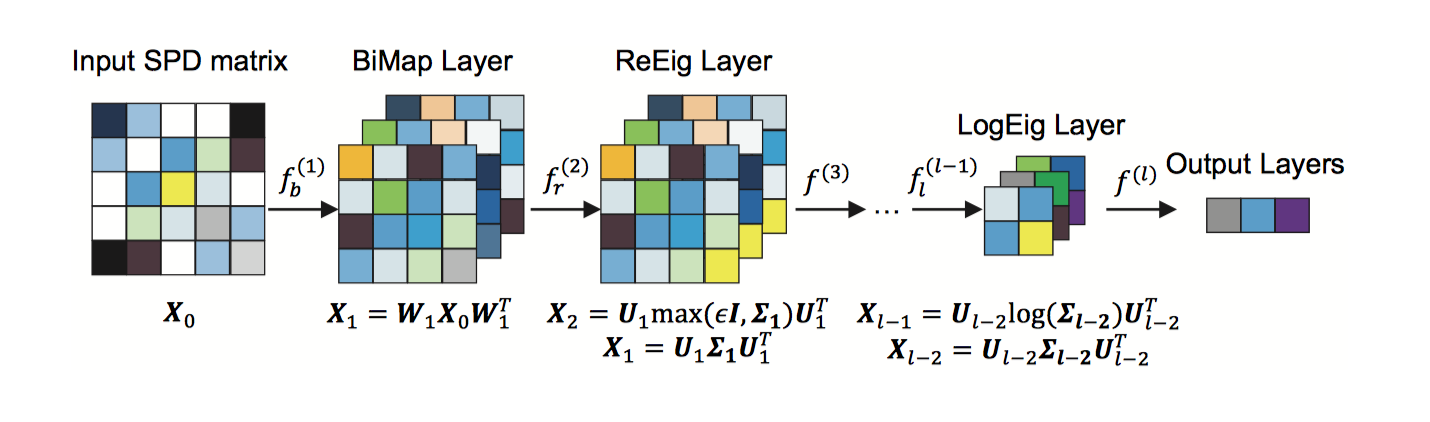
\includegraphics[scale=0.7]{pic/SPD_arch.png}
		\caption{General SPDNet architecture  \cite{Huang2016}}
		\label{fig:spd}
	\end{figure}
	
	\subsubsection*{BiMap Layer}
	
	Analogous to convolutions, BiMap layer produce linear transformation of the input SPD matrix
	\begin{equation*}
	X_k = W_k X_{k-1}W_k^T
	\end{equation*}
	The inly constraint required is that $W_k$ should be row full-rank matrix.
	
	\subsubsection*{ReEig Layer}
	The next layer corresponds to the rectified linear unit (ReLU), which aims to introduce non-linearity in the network, but instead of using restrictions on the values itself, we restrict eigenvalues of the input SPD matrix:
	
	\begin{equation*}
	X_k = U_{k-1} \max (\varepsilon I, \Sigma_{k-1})U_{k-1}^T
	\end{equation*}
	Where $X_{k-1} = U_{k-1}\Sigma_{k-1} U_{k-1}^T$ is an eigenvalue decomposition, which is defined for all SPD matrices. Contrary to a simple rectified linear unit 
	
	\subsubsection*{LogEig Layer}
	
	This layer implements projection on the tangent plane at Identity. Conceptually, it corresponds to application of Log-Euclidean kernel, discussed in \cref{sec:kernel}.
	\begin{equation*}
	X_k = U_{k-1} \log ( \Sigma_{k-1})U_{k-1}^T
	\end{equation*}
	
	
	%%%%%% Experiments %%%%%%%%%%%%%%%%
	\newpage
	\section{Experiments}
	\subsection{Data}
	
	To implement and compare different methods, introduced in the previous section, we will use dataset provided by Russian Scientific and practical psycho-neurological centre named after Z.P.Solovyov under Skoltech Biomedical Initiative program. The dataset includes 1.5T resting-state functional MRI (fMRI) of the four groups: 25 healthy controls, 25 patients with depression, 25 patients with epilepsy and 25 patients with both depression and epilepsy. For each patient $117\times 117$ symmetric positive definite matrix was created for further analysis. 
	
	To detect depression The Beck Depression Inventory (BDI), shown on \cref{fig:bdi},  was used, it is one of the most widely used tests to measure the severity of depression. Dataset also contains demographic and medical data, summarized in \cref{fig:dataset}.
	\begin{figure}[H]
		\begin{subfigure}[b]{0.48\textwidth}
			\centering
			\includegraphics[width=.95\linewidth]{pic/Age.png}
			\caption{Age distribution}
		\end{subfigure}%
		\begin{subfigure}[b]{0.48\textwidth}
			\centering
			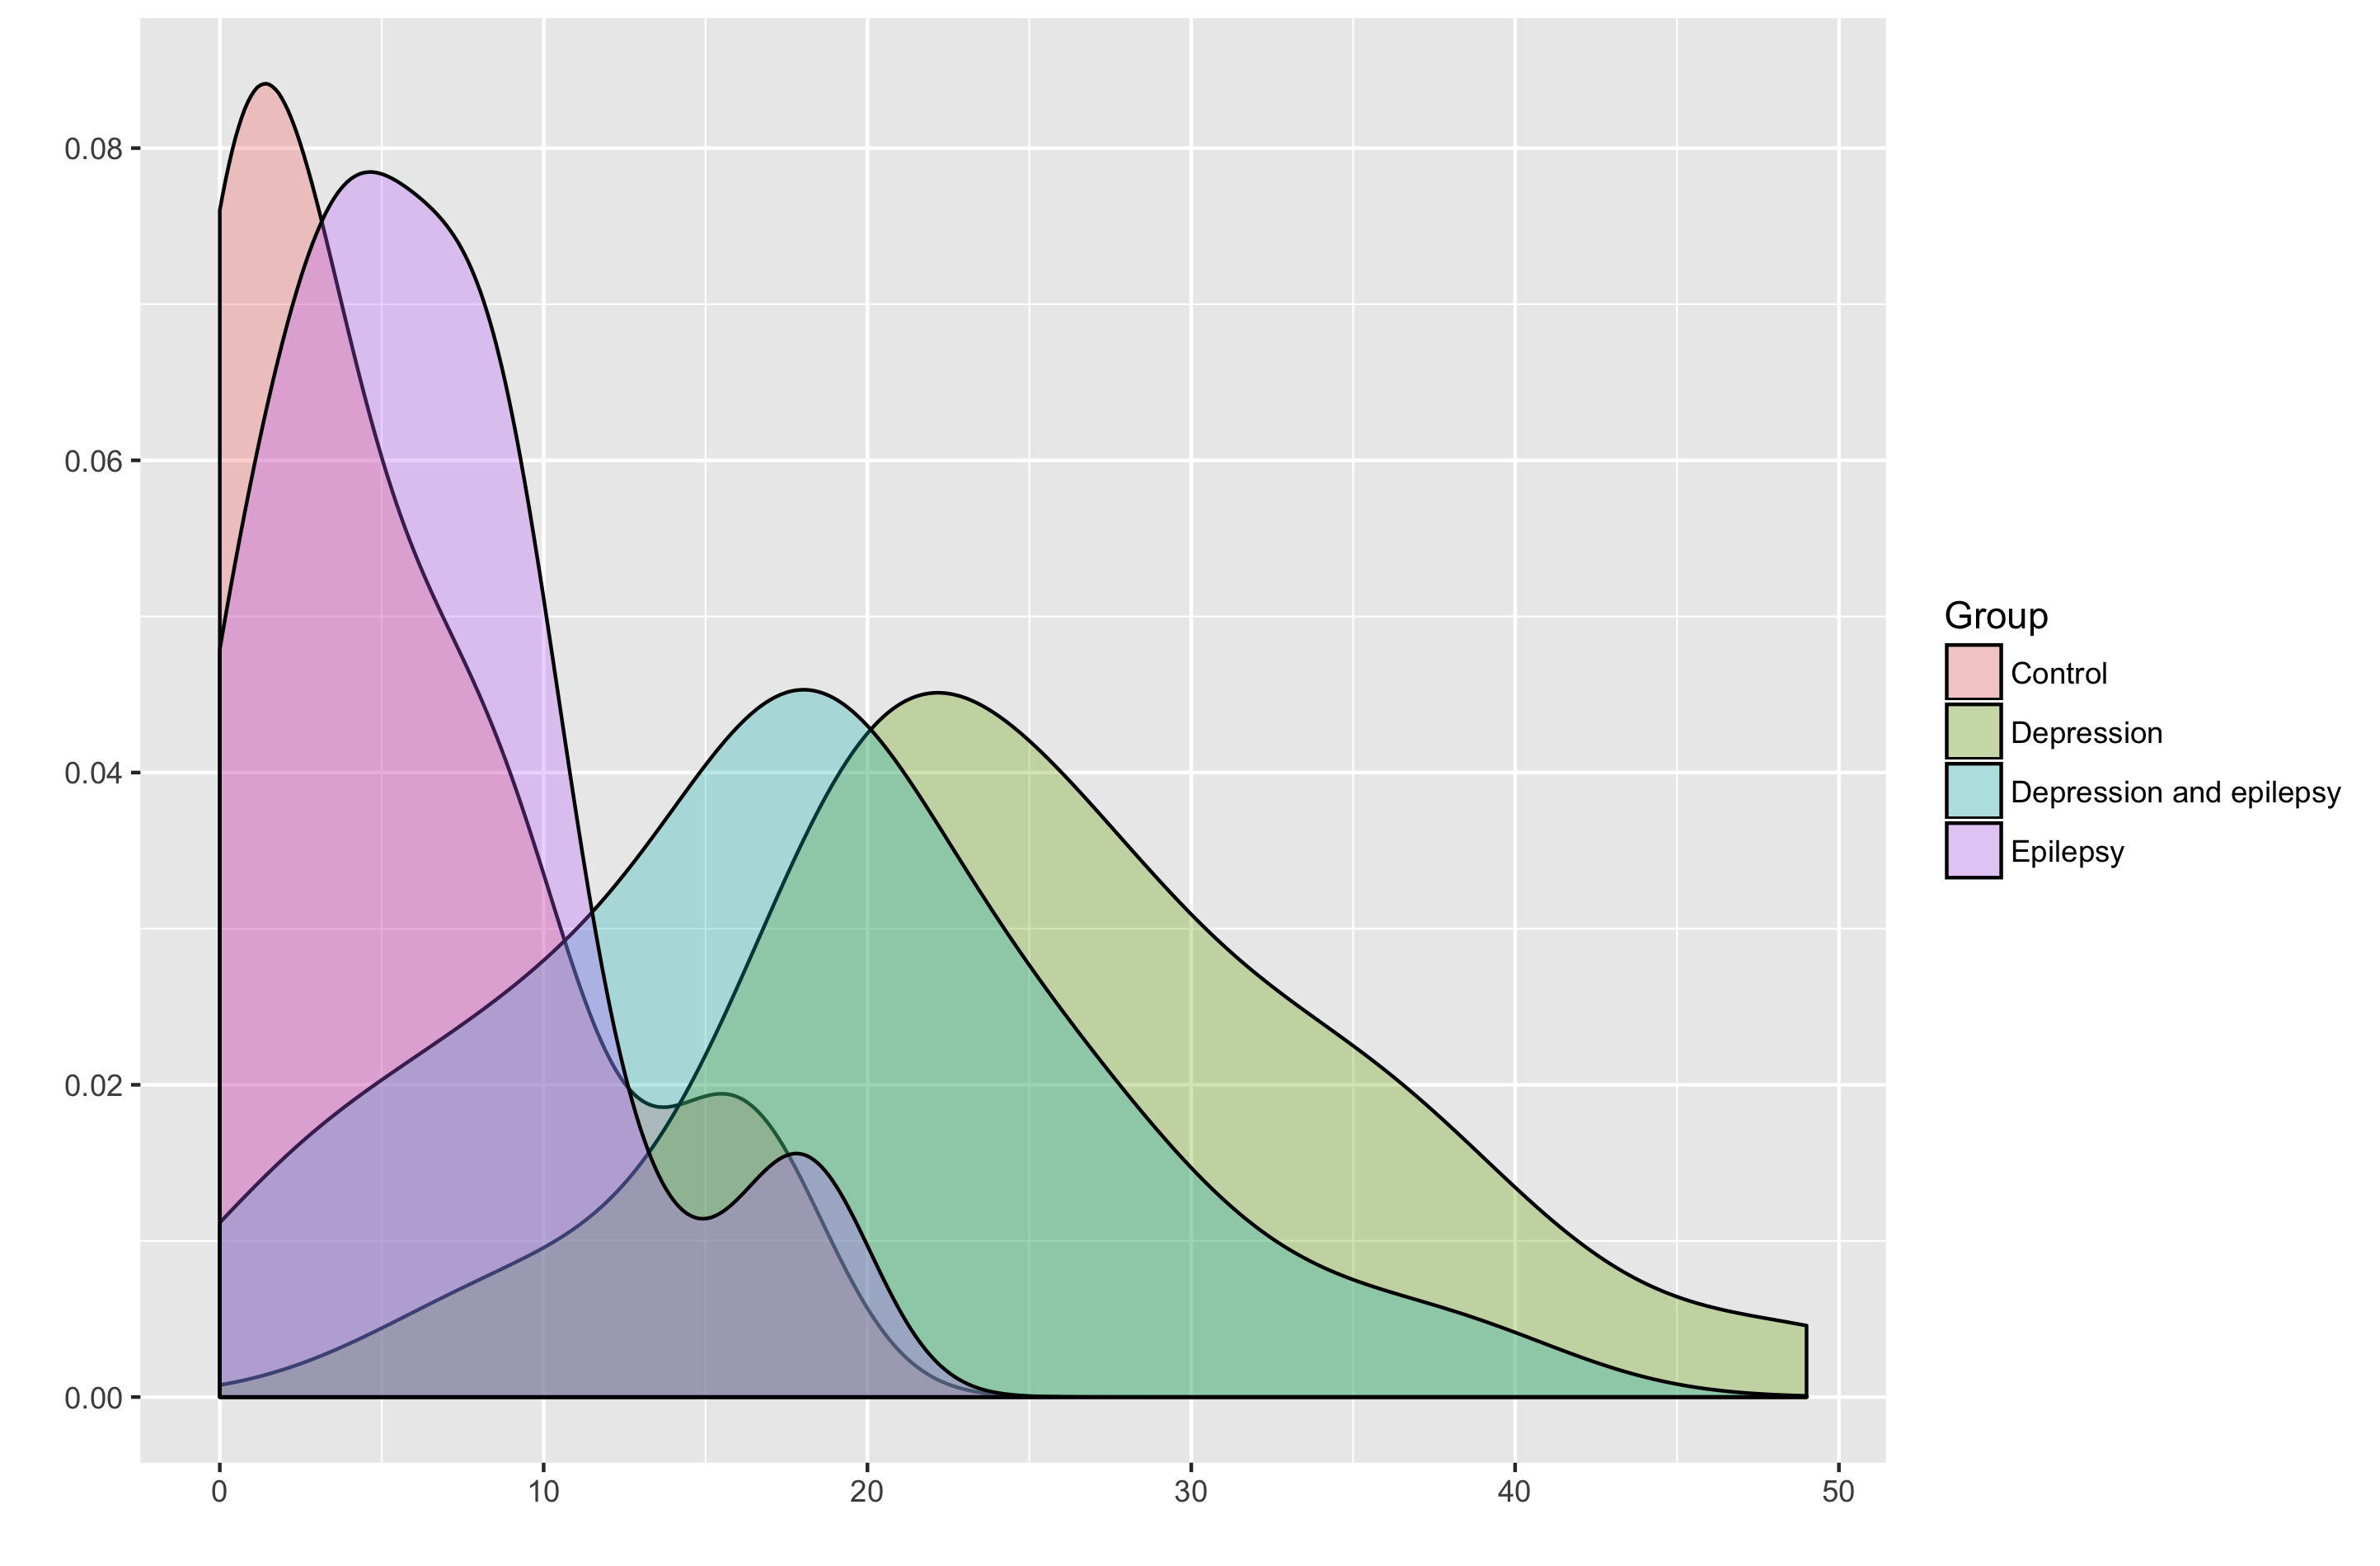
\includegraphics[width=.95\linewidth]{pic/BDI.png}
			\caption{BDI-II results}
			\label{fig:bdi}
		\end{subfigure}%
		\hfill
		\begin{subfigure}[b]{0.48\textwidth}
			\centering
			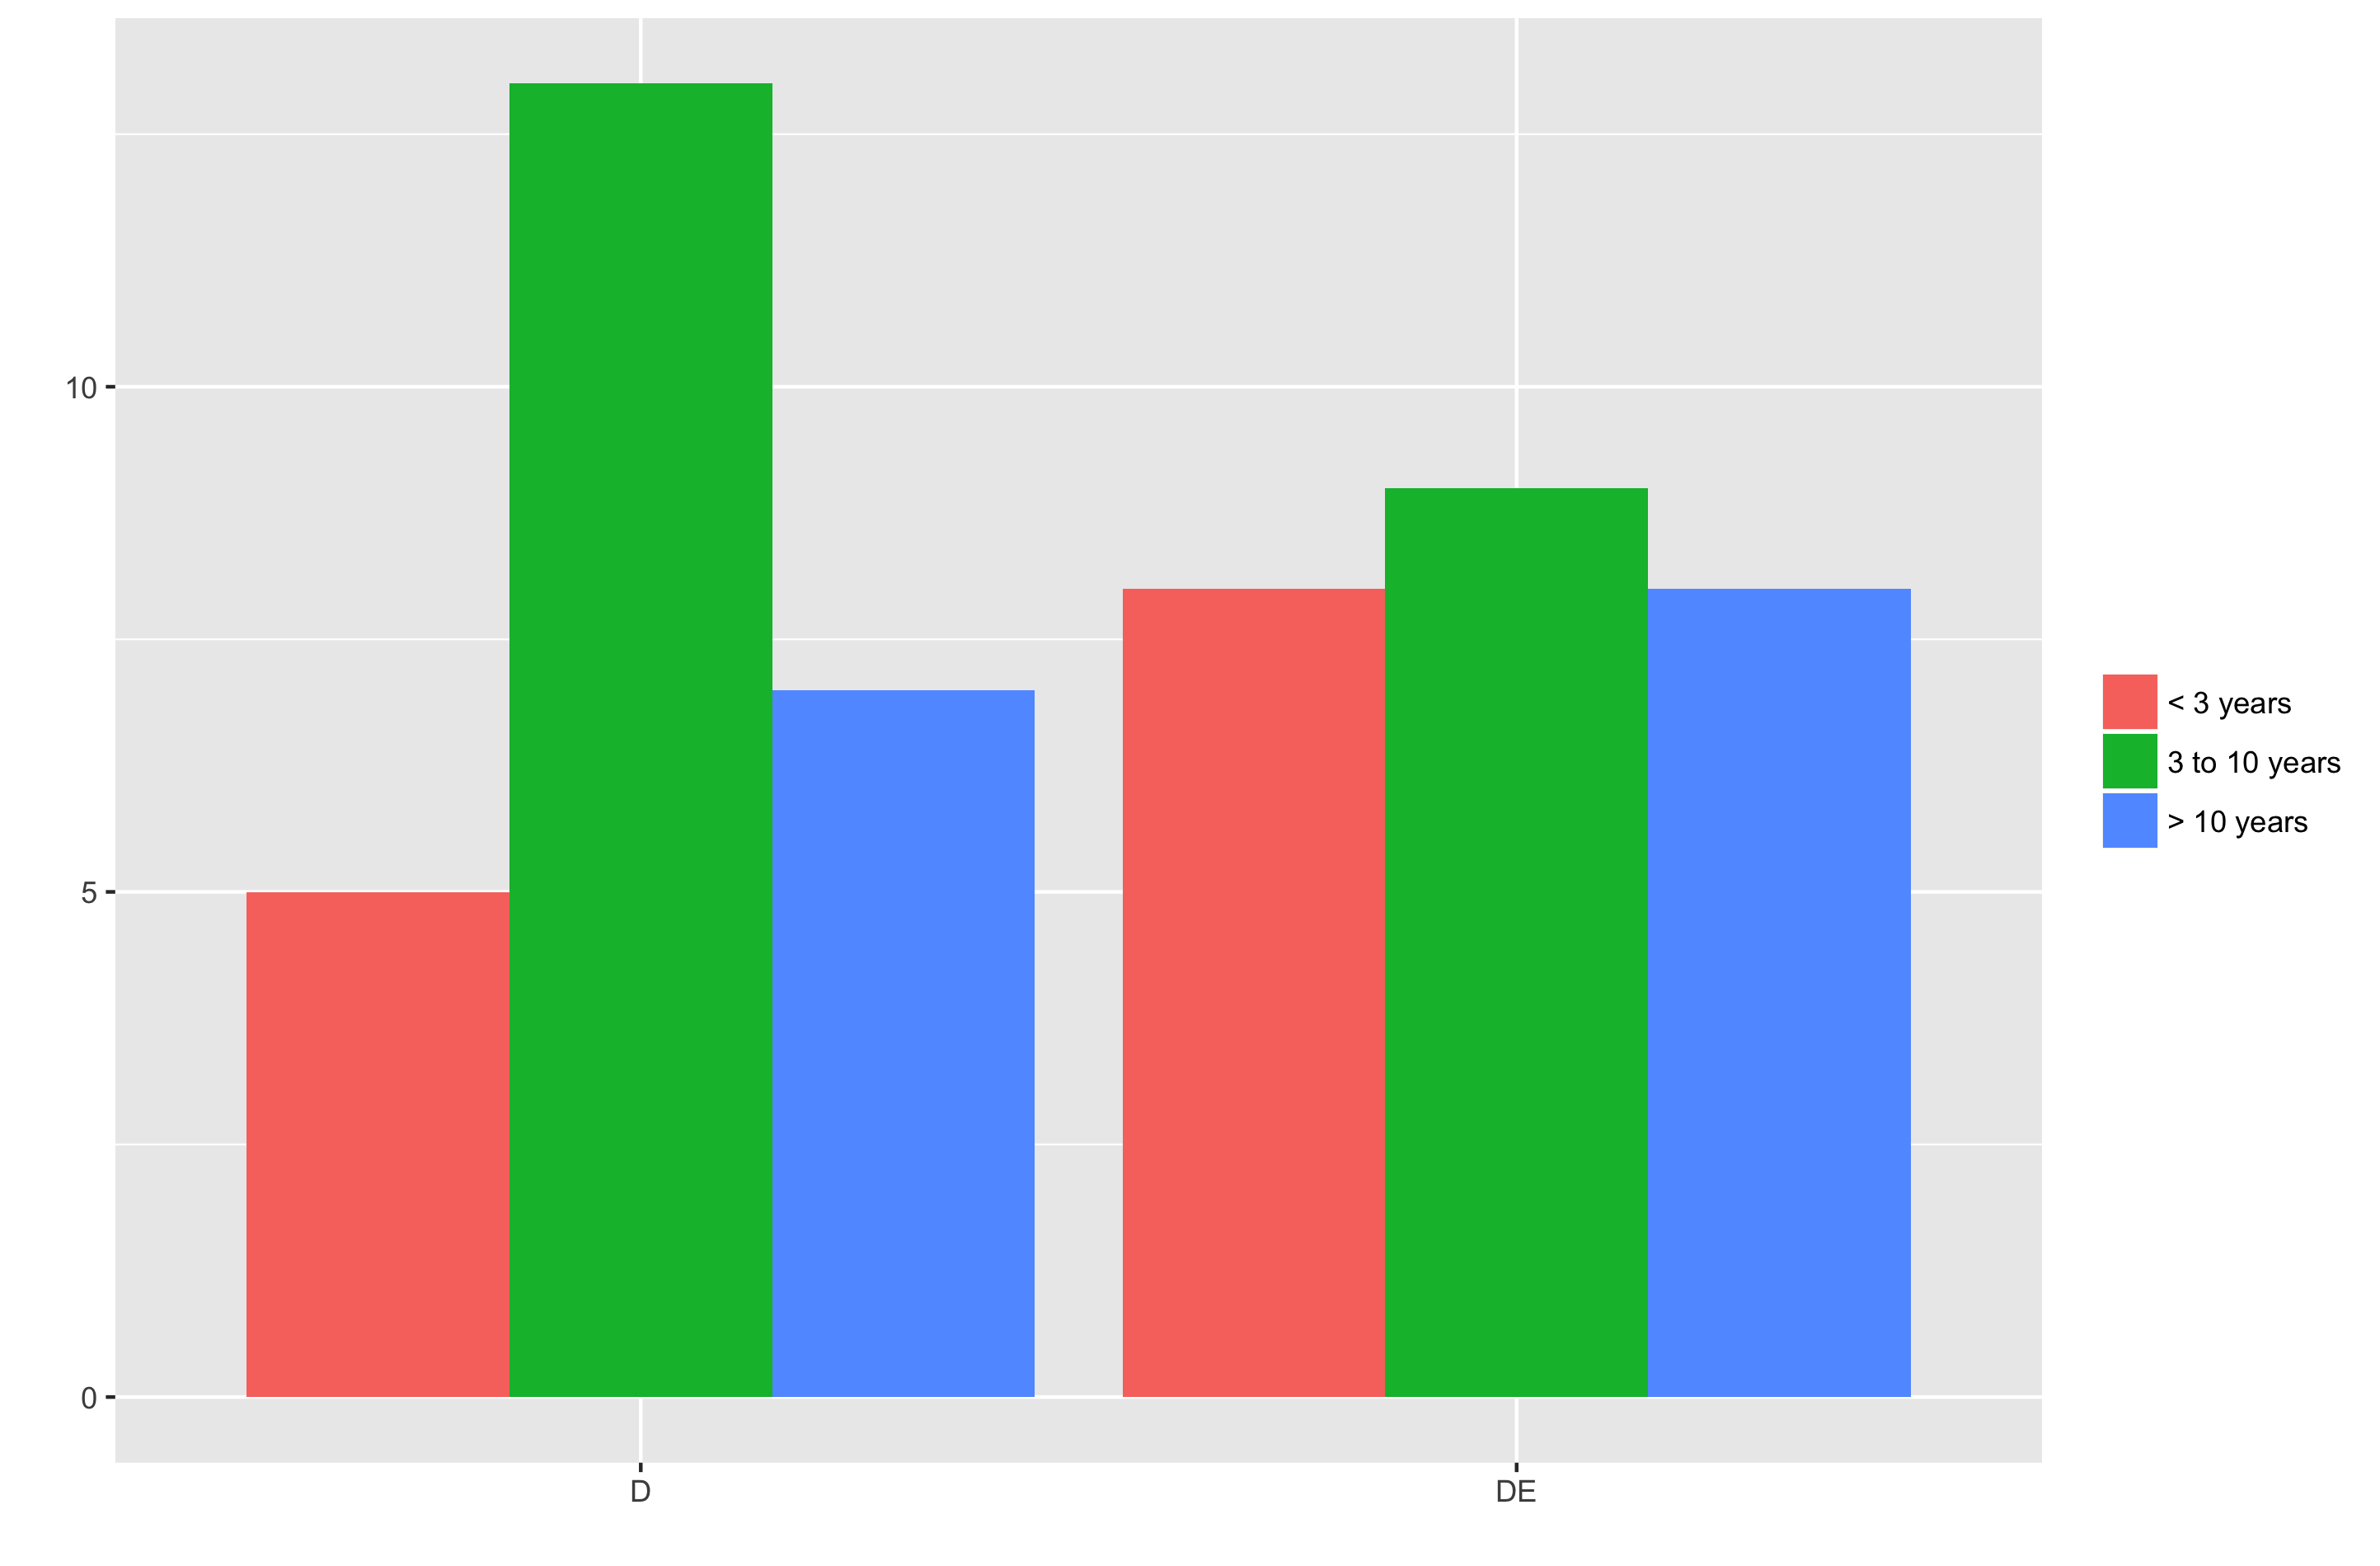
\includegraphics[width=.95\linewidth]{pic/Dep_dur.png}
			\caption{Duration of the depression}
		\end{subfigure}%
		\begin{subfigure}[b]{0.48\textwidth}
			\centering
			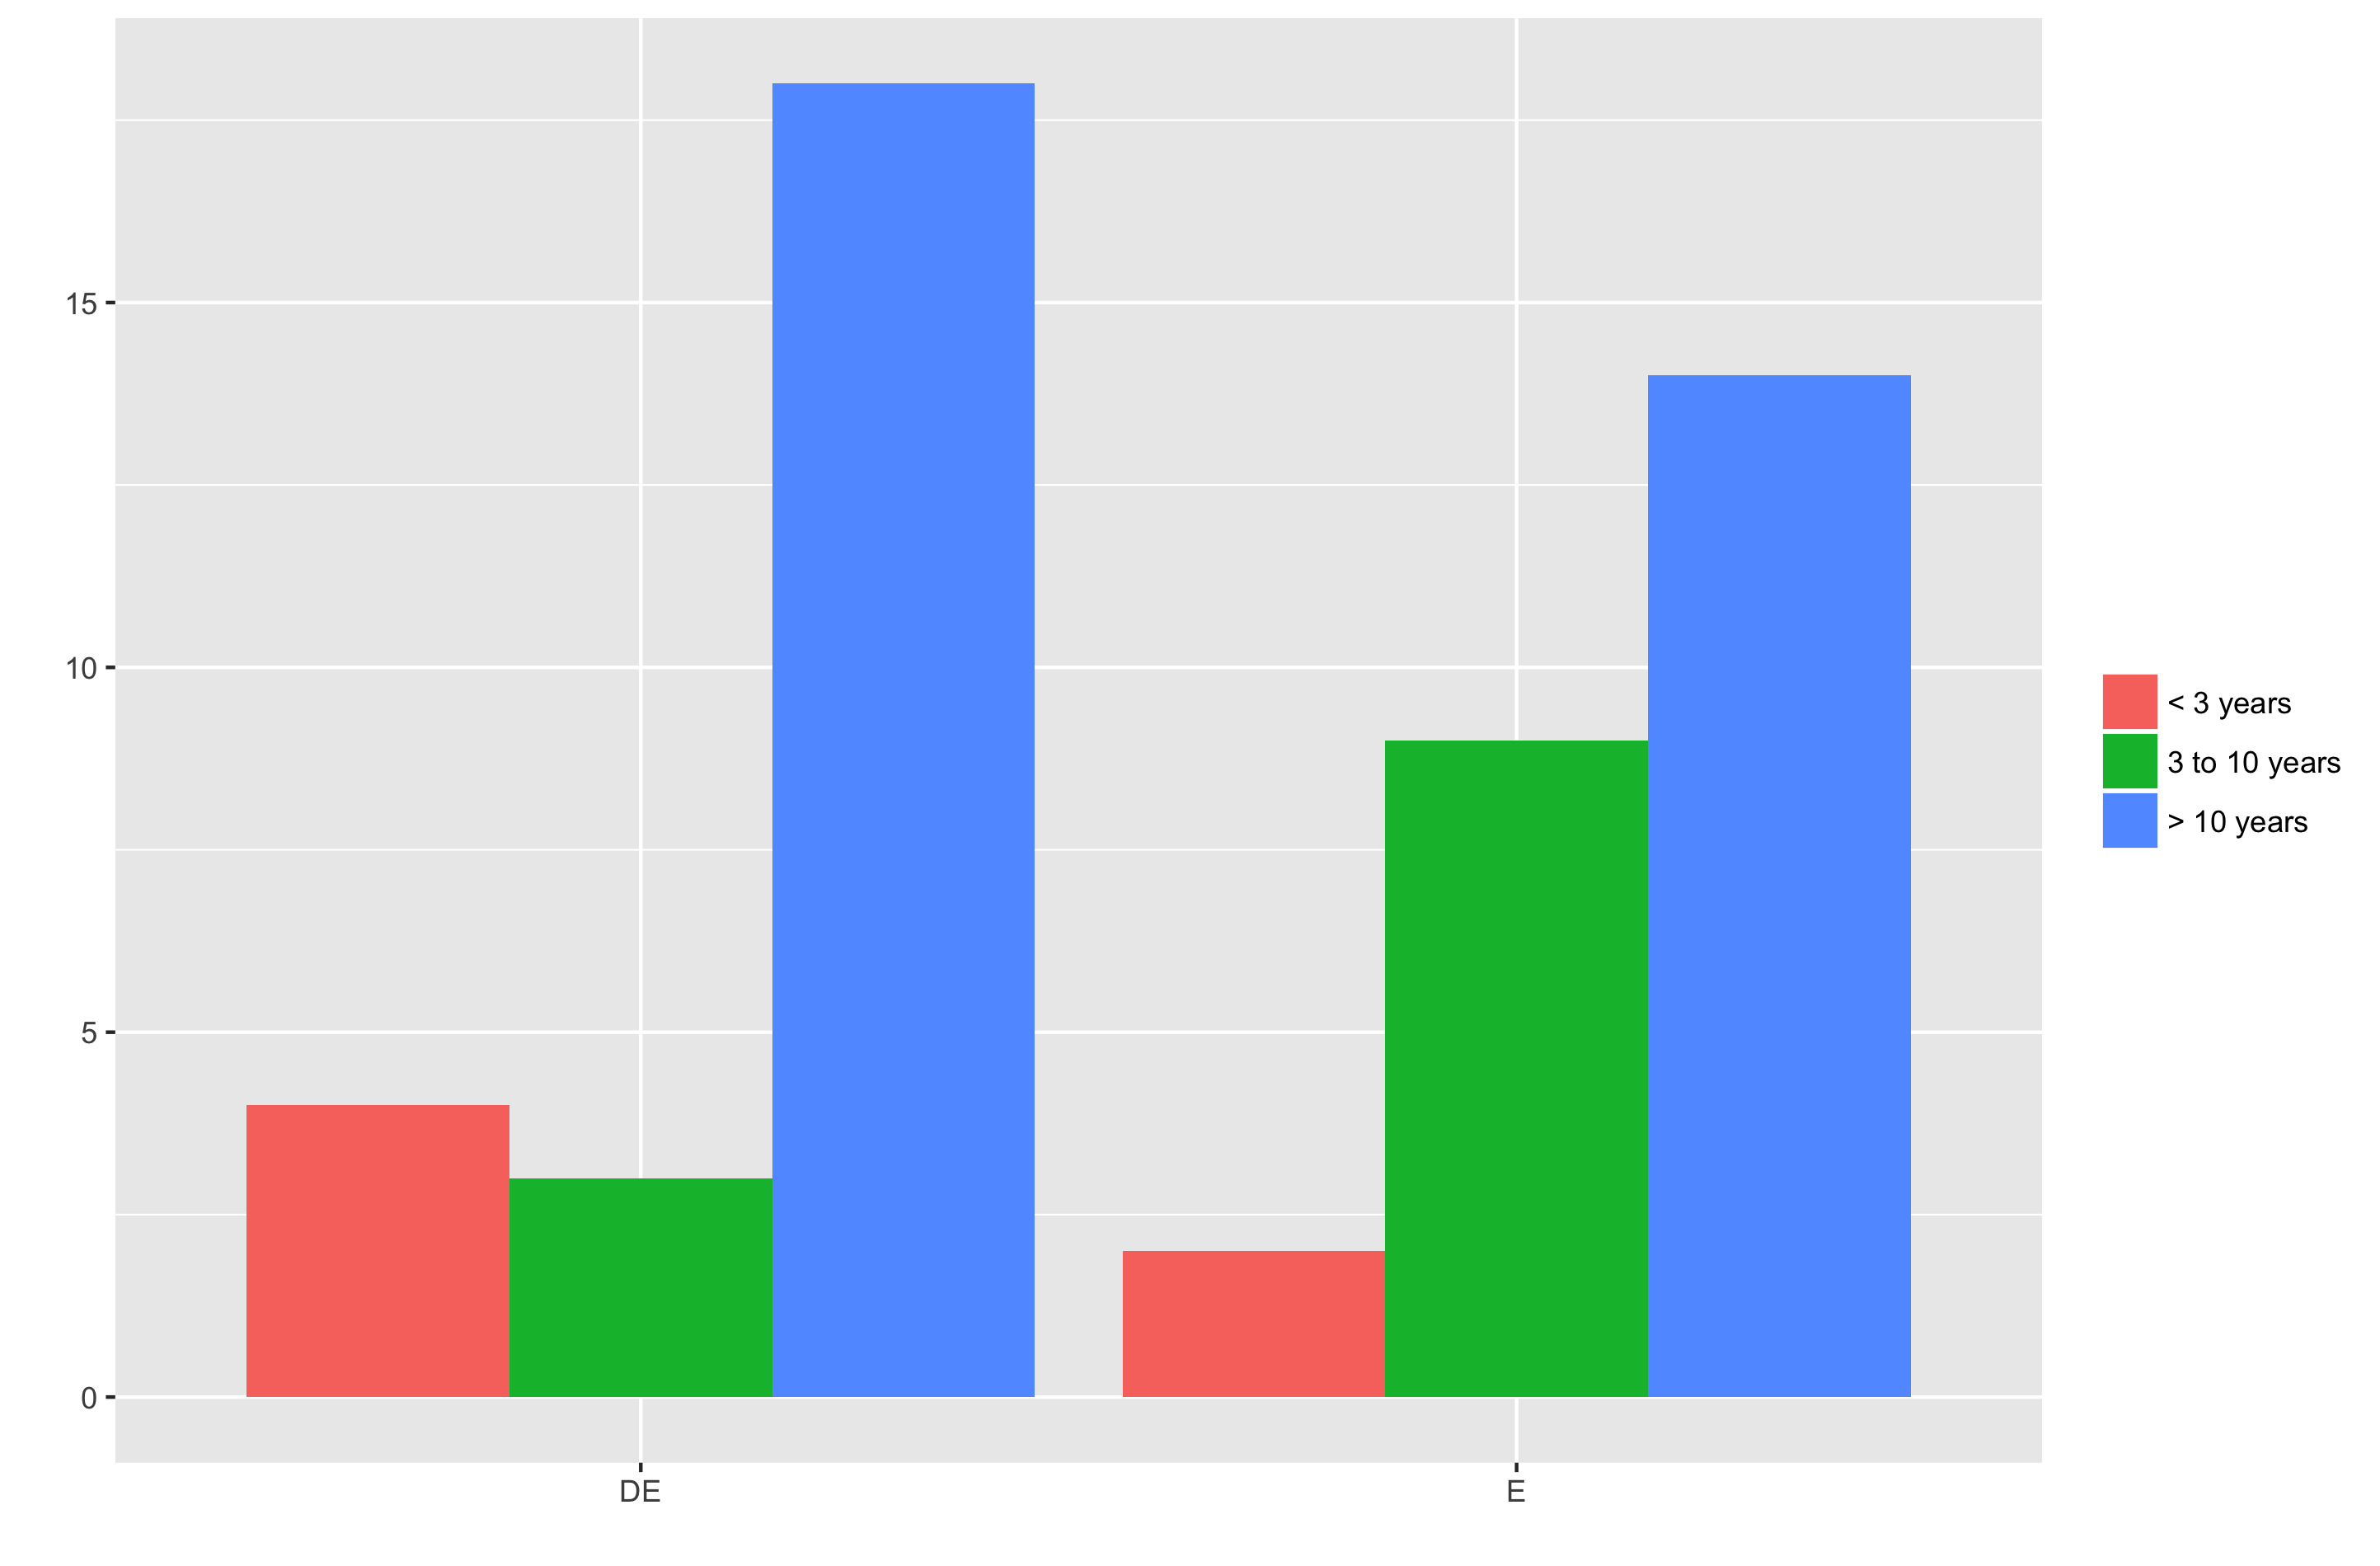
\includegraphics[width=.95\linewidth]{pic/Ep_dur.png}
			\caption{Duration of the epilepsy}
		\end{subfigure}
		\caption{Characteristics of the dataset}\label{fig:dataset}
	\end{figure}
	
	Overall, 8 classification problems were distinguished:
	\begin{itemize}
		\item Depression detection, 100 patients \textbf{(D+DE vs E+C)}
		\item Epilepsy detection, 100 patients \textbf{(E+DE vs D+C)}
		\item Depression detection, 50 patients \textbf{(D vs C)}
		\item Epilepsy detection, 50 patients \textbf{(E vs C)}
		\item Depression detection in patients with epilepsy, 50 patients \textbf{(DE vs E)}
		\item Epilepsy detection in patients with depression, 50 patients \textbf{(DE vs D)}
		\item Temporal lobe epilepsy detection, 81 patients \textbf{(TLE (31) vs C+D (50))}
		\item Temporal lobe epilepsy detection, 56 patients \textbf{(TLE (31) vs C (25))}
	\end{itemize}
	
	
	
	\subsection{Models}
	
	For each classification problem above four models have been estimated, with hyperparameters selected with grid search on 10-fold stratified cross-validation. Below parameters and their possible values are discussed in more detail.
	\subsubsection*{Minimum distance to mean (MDM)}
	\begin{table}[!h]
		\begin{center}
			\begin{tabular}{ l | l  }
				%\hline
				%\multicolumn{4}{ c |}{\textbf{kNN parameters}}  & \textbf{Equipo} \\ 
				%\cline{1-4}
				Parameter &  Values \\ \hline
				Metric &   [`riemann`, `logeuclid`, `euclid'`]\\  
				%\hline
			\end{tabular}
			\caption{Parameter grid for MDRM}
			\label{T:mdrm_par}
		\end{center}
	\end{table}
	
	In this case, only one hyperparameter needs to be chosen: type of metric used for centroid and distance estimation. If we choose \texttt{`riemann`}, then MDRM from \cref{sec:classification} is estimated. 
	
	\subsubsection*{kNN}
	
	\begin{table}[!h]
		\begin{center}
			\begin{tabular}{ l | l }
				%\hline
				%\multicolumn{4}{ c |}{\textbf{kNN parameters}}  & \textbf{Equipo} \\ 
				%\cline{1-4}
				Parameter &  Values \\ \hline
				Number of neighbors &   1 to 50 with step 5 (1 to 25 for smaller sample)\\ 
				Metric &   [`riemann`, `logeuclid`, `euclid'`]\\ 
				%\hline
			\end{tabular}
			\caption{Parameter grid for k-nearest neighbors}
			\label{T:kNN_par}
		\end{center}
	\end{table}
	
	In this model, we have two hyperparameters. First one, \texttt{number of neighbors}, is a usual parameter for this method, it controls the number of nearest objects, used to identify the class of the current object. Another one appeared, because we again want to compare the Riemannian distance to the Euclidean one.
	
	\subsubsection*{Support Vector Machine}
	
	When it comes to SVM, there are two possible ways to include Riemannian geometry in the model. One may implement so-called kernel SVM, using \cref{eq:kernel}. Another approach, implemented in this work, is to firstly map all the data into the tangent plane and then apply SVM algorithm to the obtained vectors. as we can see from \cref{eq:kernel}, there is a closed form equation for this mapping:
	\begin{equation*}
	\tilde{P}_i = \log (P^{*-\frac12}P_i P^{*-\frac12})
	\end{equation*}
	The benefit of this approach is that we may further apply kernel SVM on top of the projected data.  As shown in \cref{T:SVM_par}, two different kernels were applied. For \texttt{`rbf`} kernel parameter \texttt{Gamma} controls how much influence a single training example has. Regularization coefficient, penalty parameter of the error term, is also chosen from the grid. 
	\begin{table}[!h]
		\begin{center}
			\begin{tabular}{ l | l  }
				%    \hline
				%\multicolumn{4}{ c |}{\textbf{SVM parameters}}  & \textbf{Equipo} \\ 
				%\cline{1-4}
				Parameter &  Values\\ \hline
				kernel & [`linear`, `rbf`] \\
				Regularization coefficient C &  [1e-04, 1e-2, 1, 10, 100]\\ 
				gamma & [1e-04, 1e-2, 1, 10] \\ 
				Metric &   [`riemann`, `logeuclid`, `euclid'`]\\ 
				%\hline
				
			\end{tabular}
			\caption{Parameter grid for SVM}
			\label{T:SVM_par}
		\end{center}
	\end{table}
	
	\subsubsection*{Logistic Regression}
	
	Finally, logistics regression was estimated with different metrics and regularization coefficients, presented in \cref{T:LR_par}.
	\begin{table}[H]
		\begin{center}
			\begin{tabular}{ l | l }
				%            \hline
				%\multicolumn{4}{ c |}{\textbf{SVM parameters}}  & \textbf{Equipo} \\ 
				%\cline{1-4}
				Parameter &  Values\\ \hline
				Regularization coefficient C &  [1e-04, 1e-2, 1, 10, 100]\\ 
				Metric &   [`riemann`, `logeuclid`, `euclid'`]\\ 
				%\hline
			\end{tabular}
			\caption{Parameter grid for LR}
			\label{T:LR_par}
		\end{center}
	\end{table}
	
	\subsection{Results}
	
	\subsubsection*{Kernel Methods and classification on manifold}
	Finally, accuracy and area under ROC-curve for the best models are presented in \cref{T:res}. The grid search was performed on stratified cross-validation. For models classification problems with 100 observations 10-folds cross-validation was applied, while for ones with smaller sample 5-folds were used. 
	
	
	\begin{table}[H]
		\centering
		\begin{tabular}{l|lllll}
			& Best Model &  Metric & Accuracy& ROC-AUC   \\ \hline
			\textbf{E/no E} &  SVC &riemann &  0.57(0.17)   &   0.57  \\
			\textbf{D/no D} &   SVC& riemann   & \textbf{0.68(015)}  & 0.70    \\  
			\textbf{E/C} &    SVC &riemann  & 0.59(0.13)  & 0.70    \\ 
			\textbf{D/C} &    LR & riemann & \textbf{0.67(0.22) } & 0.70    \\ 
			\textbf{TLE/no E} &    LR &euclid & 0.62(0.17)  & 0.60    \\ 
			\textbf{TLE/C} &    SVC& riemann  & 0.57(0.15) & 0.57     \\ 
			\textbf{DE/E} &    SVC  &riemann &\textbf{0.70(0.18) }& 0.77   \\ 
			\textbf{DE/D} &    SVC & riemann & \textbf{0.73(0.17) } & 0.70    \\ 
		\end{tabular}
		\caption{Accuracy of the best models on cross-validation}
		\label{T:res}
	\end{table}
	
	
	As it was already mentioned, when obtaining adjacency matrix for the graph, correlation threshold was applied. An optimal value for this threshold was chosen together with other hyperparameters from values $[0.1, 0.2, 0.3]$. The sensitivity of ROC-AUC value to the changes in threshold for the four best models is depicted on \cref{fig:thr}. It can be seen that one could not obtain significantly better results by tuning this hyperparameter.
	
	\begin{figure}[H]
		\begin{subfigure}[b]{0.48\textwidth}
			\centering
			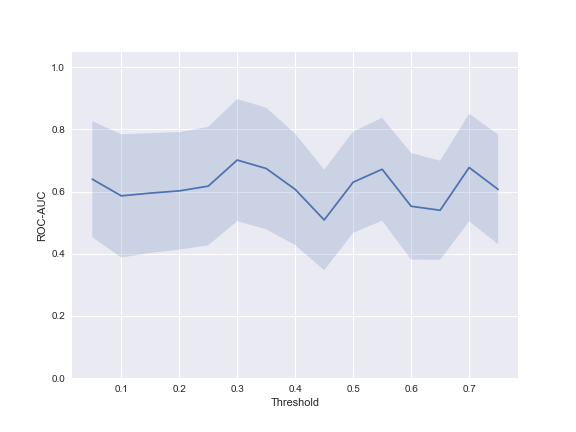
\includegraphics[width=\linewidth]{pic/DC_th.png}
			\caption{Depression vs Control}
			\label{fig:bdi}
		\end{subfigure}
		\begin{subfigure}[b]{0.48\textwidth}
			\centering
			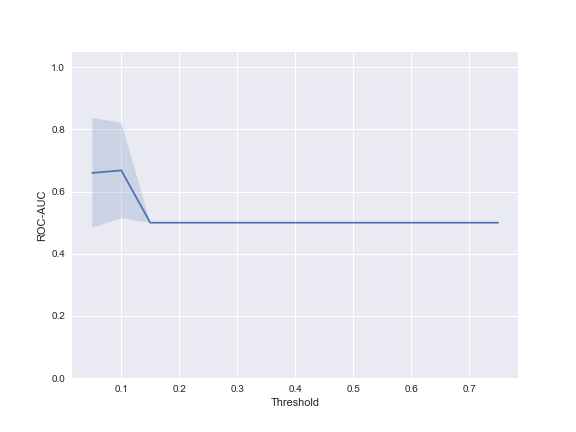
\includegraphics[width=\linewidth]{pic/D_th.png}
			\caption{Depression vs No depression}
		\end{subfigure}%
		\hfill
		\begin{subfigure}[b]{0.48\textwidth}
			\centering
			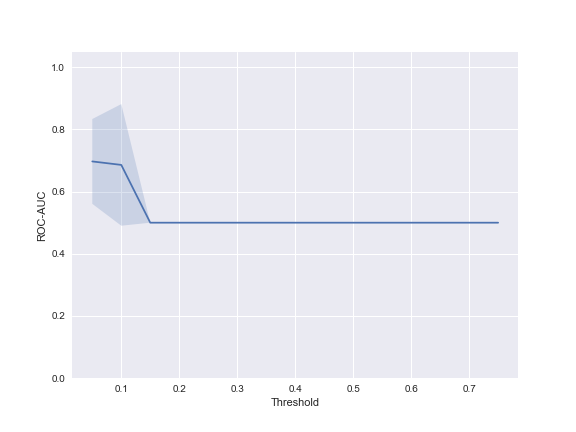
\includegraphics[width=\linewidth]{pic/DE_E_th.png}
			\caption{Depression with epilepsy vs epilepsy}
		\end{subfigure}%
		\begin{subfigure}[b]{0.48\textwidth}
			\centering
			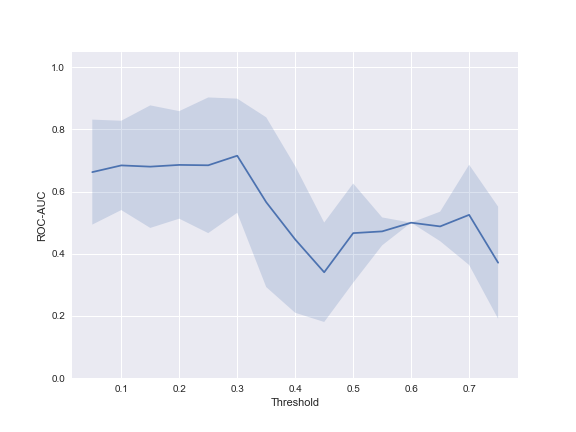
\includegraphics[width=\linewidth]{pic/DE_D_th.png}
			\caption{Depression with epilepsy vs depression}
		\end{subfigure}
		\caption{Sensitivity to threshold changes}
		\label{fig:thr}
	\end{figure}
	
	
	\subsubsection*{Riemannian Network}
	
	The Riemannian network was also fitted to the described problem and dataset. Implementation from the original paper on Matlab is available on \href{https://github.com/zzhiwu/SPDNet}{Gihub}. Unfortunately, due to the extremely small dataset, there were no reasonable results obtained.
	
	\begin{figure}[H]
		\begin{subfigure}[b]{0.48\textwidth}
			\centering
			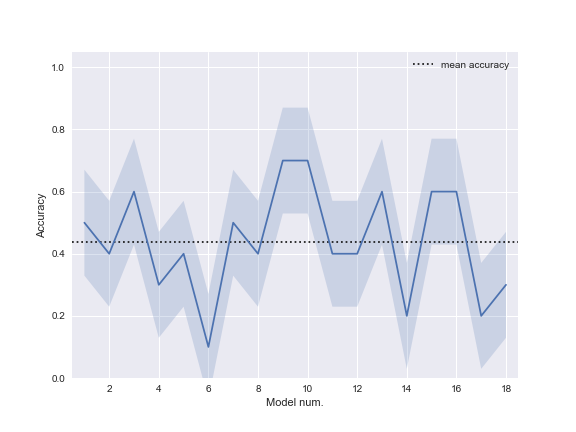
\includegraphics[width=\linewidth]{pic/Rnet_dep.png}
			\caption{Depression vs Control}
			\label{fig:bdi}
		\end{subfigure}
		\begin{subfigure}[b]{0.48\textwidth}
			\centering
			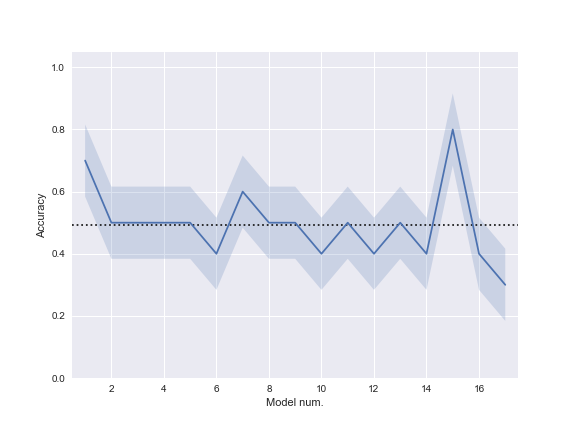
\includegraphics[width=\linewidth]{pic/Rnet_ep.png}
			\caption{Epilepsy vs Control}
		\end{subfigure}%
		\caption{SPDnet accuracy on cross-validation}
		\label{fig:spdnet_acc}
	\end{figure}
	When using minimal architecture, with two BiMap + ReEig layers and one LogEig layer, results are very unstable and on average close to the random choice with accuracy $\frac12$, as shown of the \cref{fig:spdnet_acc}. In most cases, network was not able to learn anything useful from the data. One of the best results with accuracy 0.7 on the validation set is shown on the \cref{fig:spdnet_train}. But again, this is a very unstable, as seen from the total statistics. 
	
	\begin{figure}[H]
		\centering
		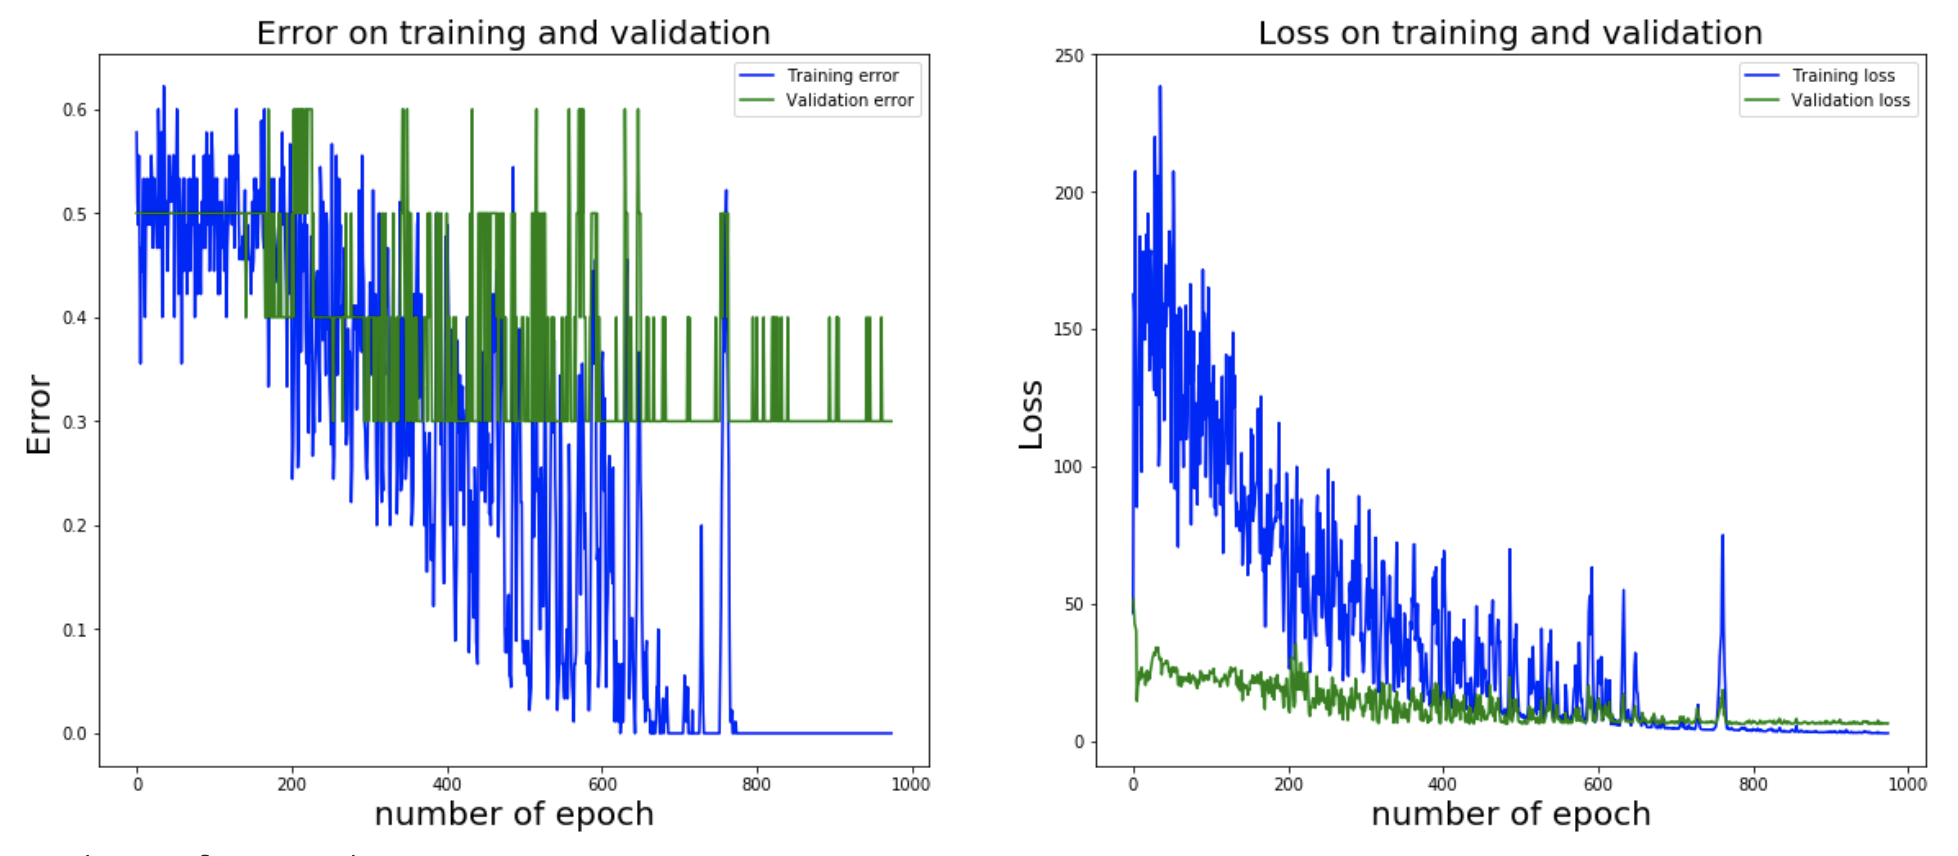
\includegraphics[width=\linewidth]{pic/depr.png}
		\caption{Training of the SPDnet for D/no D problem}
		\label{fig:spdnet_train}
	\end{figure}
	
	Extra hyperparameter tuning did not improve the result. In order to make sure, that network architecture was correctly transferred from Matlab to python and applied to fMRI data the same procedure was repeated with ABIDE dataset\cite{Craddock2013}. It contains preprocessed fMRI of 539 individuals suffering from ASD and 573 typical controls. When training the same network on this dataset (see \cref{fig:spdnet_abide}), the more positive picture can be seen. Moreover, the result is stable when validating it on cross-validation
	
	\begin{figure}[H]
		\centering
		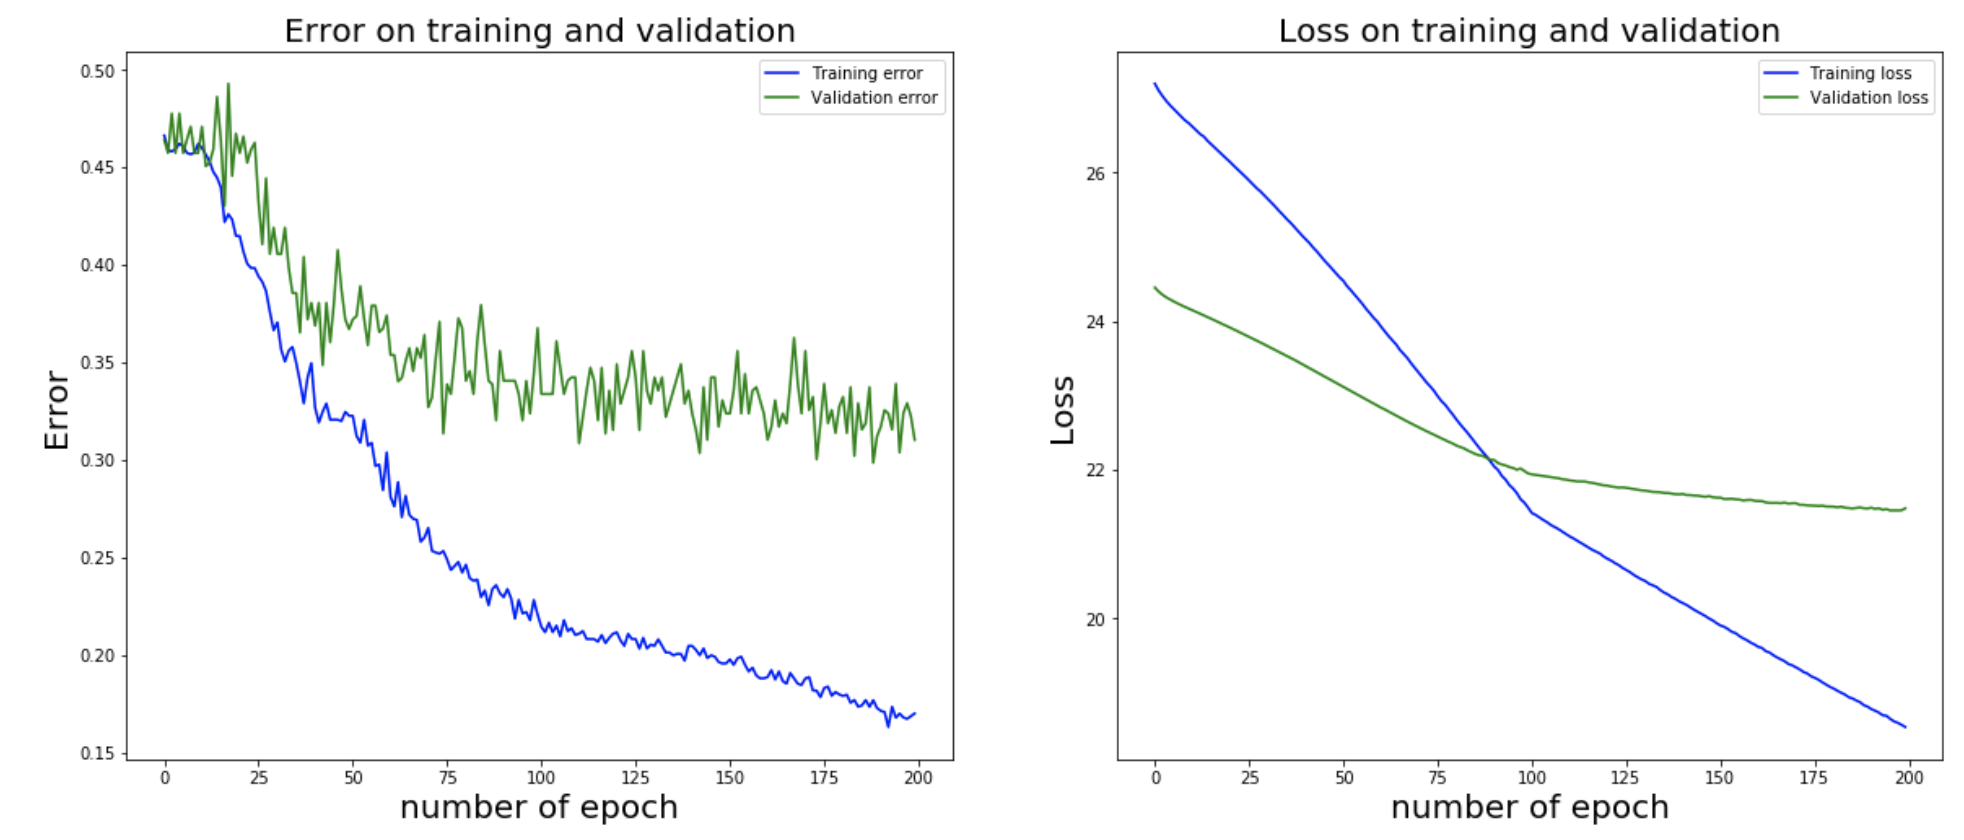
\includegraphics[width=\linewidth]{pic/abide.png}
		\caption{Training of the SPDnet on ABIDE dataset}
		\label{fig:spdnet_abide}
	\end{figure}
	
	
	\section{Summary}
	This work extensively discusses machine learning techniques which can be applied to classification of SPD matrices, taking into account the Riemannian structure of their space. Affine-invariant metric and distances are used to adopt such methods as k-nearest neighbours, support vector machines or even neural network to this special data. Result shows, that utilization of Riemannian metric in most cases outperform Euclidean one on the conventional machine learning algorithms. However, in order to get reasonable results on the SPDnet, a larger dataset is needed.
	
	%%%%%% Bibliography %%%%%%%%%%%%%%%%
	\newpage
	\bibliography{Collection}{}
	\nocite{*}
	\bibliographystyle{abbrv}
	
\end{document}
